\documentclass[conference]{IEEEtran}

\usepackage{hyperref}
\usepackage{amsmath}
\usepackage{booktabs}
\usepackage{enumitem}
\usepackage{cite}
\usepackage{pgfplots}
\usepackage{microtype}

\usepgfplotslibrary{groupplots}
\pgfplotsset{compat=1.18}

\hyphenpenalty=500
\exhyphenpenalty=200
\doublehyphendemerits=100000
\finalhyphendemerits=5000

\title{Arrival-Time KV Materialization for LLM Serving}

\author{\IEEEauthorblockN{Anonymous Authors}}

\begin{document}
\maketitle

\newcommand{\HeuristicMeanTTFT}{10.782}
\newcommand{\HeuristicPNineFiveTTFT}{22.161}
\newcommand{\OracleMeanTTFT}{9.912}
\newcommand{\OraclePNineFiveTTFT}{21.1}


\begin{abstract}
Reusable KV state can reduce prefill work, but loading and adapting that state
also consumes time and bandwidth. We study the request-arrival decision among
full prefix reuse, block-aligned partial reuse, and recomputation. A lightweight
controller estimates saved prefill work against realization cost and exposes
the action that the runtime actually executes, rather than reporting cache hits
alone. An offline cost-model study over 1,296 requests from 25 workload cases
finds that full reuse remains the best mean-latency policy in 18 cases and that
the oracle selects partial reuse for only 71 requests. Thus partial reuse is a
workload-specific option, not a universal improvement. A prototype vLLM path
implements block-aligned segmentation and records action realignment. The
online results in this draft are descriptive single runs; they validate the
runtime path but do not establish a statistically significant speedup.
\end{abstract}

\begin{IEEEkeywords}
LLM serving, KV cache, prefix reuse, materialization control, time to first token
\end{IEEEkeywords}

\section{Introduction}
Recent LLM serving systems increasingly rely on prefix reuse, prompt caching,
and reusable KV state to reduce prefill cost. However, a reusable prefix is not
equivalent to a free latency reduction. In multi-GPU settings, reusable state
may reside on another worker, may require transfer through interconnect or host
memory, and may need partial rematerialization before decoding can start. As a
result, the serving system faces a control problem: when a request arrives and
some reusable state exists, how much of that state should be realized now?

Recent disaggregated and remote-KV serving efforts, including DistServe and
Mooncake~\cite{distserve2024,mooncake2025}, make this cost visible rather than
hiding it behind a monolithic ``cache hit'' abstraction. Once reuse requires
transport, re-layout, or partial reconstruction, the runtime needs a policy
that decides whether realizing the reusable state is worth the startup cost.

That decision is structurally closer to selective materialization than to a
binary cache-hit classifier. A serving stack is not merely asking whether
reuse exists; it is asking whether a reusable state fragment should be
materialized now, how much of it should be materialized, and when recomputing
the remainder is cheaper. This perspective is inspired by selective
materialization work in other domains, where the key systems question is not
``can this state be reused?'' but ``is materializing it worth the cost under
the current workload and resource conditions?''~\cite{leap2024}.

We focus on a narrow but practically important control point: request-arrival
KV materialization. Instead of treating reuse as a binary
choice, we study a three-action decision surface. The controller can fully
materialize the reusable prefix, partially materialize only a profitable
segment, or ignore the reusable state and recompute the prompt from scratch.
This formulation is intentionally orthogonal to placement, admission, and
online memory-evolution policy. Placement affects where reusable state resides;
admission affects which work enters the system; memory evolution affects how
state is written, retained, or retired over time. Our question begins after
reusable state is already available and asks whether realizing it at request
arrival is worth the cost.

The systems hypothesis is straightforward: the best action depends on the
tradeoff between recomputation work and realization overhead. Realization
overhead can include transfer latency, bytes moved, device memory pressure, and
stitching cost. Recompute cost depends on prompt length, model throughput, and
request urgency. Because these factors vary across workloads, a serving stack
needs an explicit materialization controller instead of a fixed ``always reuse''
rule.

In contrast to a broad scheduler redesign, this paper targets one measurable
hook and keeps placement, admission, and eviction unchanged. We make three
contributions:
\begin{itemize}[leftmargin=1.5em]
\item a three-action formulation of arrival-time KV realization;
\item a block-aligned vLLM mechanism that separates requested and executed
actions; and
\item an evaluation that identifies a narrow partial-reuse region and reports
online path behavior without promoting modeled results to measured speedups.
\end{itemize}

\section{Problem Formulation}
We study a single-hook decision problem at request arrival. For each incoming
request, the runtime observes a candidate reusable prefix together with signals
about prefix length, estimated recomputation work, and estimated realization
cost. The controller then chooses one of three actions:

\begin{itemize}[leftmargin=1.5em]
\item \texttt{full\_reuse}: materialize the full reusable prefix,
\item \texttt{partial\_reuse}: materialize only a prefix segment and recompute the rest,
\item \texttt{recompute}: ignore reusable state and run the prompt path from scratch.
\end{itemize}

This decision surface is deliberately narrow. It avoids conflating multiple
control layers and makes the evidence interpretable: if the controller helps,
the gain comes from better request-arrival materialization decisions rather
than from a hidden change in scheduler, placement, or eviction behavior.

\subsection{Signals and Objective}
The controller reasons over a small signal set: reusable prefix length,
estimated transfer latency, estimated recomputation latency, queue pressure,
and a confidence estimate for whether the candidate reusable state is likely to
produce useful saved work. The objective is to minimize startup latency,
represented primarily by TTFT, while keeping realized KV traffic proportional
to actual benefit.

We use these signals through a simple utility view. For a candidate action
$a$, the controller estimates the startup benefit from avoided recomputation,
then subtracts realization-side overheads such as transfer, stitching, and
pressure amplification. Conceptually,
\[
U(a) = B_{\text{recompute}}(a) - C_{\text{realize}}(a)
- P_{\text{pressure}}(a).
\]
The controller selects the action with the largest non-negative utility.
Under this view, \texttt{full\_reuse} corresponds to materializing the whole
reusable prefix, \texttt{recompute} corresponds to rejecting materialization,
and \texttt{partial\_reuse} corresponds to selecting only a profitable prefix
segment when early reuse has positive value but the tail does not.

This formulation is intentionally lightweight: it is not presented as a
globally optimal estimator, but as the minimal abstraction needed to compare
three actions on equal footing and to expose where runtime support is still
missing.

\subsection{Why Partial Reuse Matters}
The partial action is the key difference between a binary reuse controller and
a materialization controller. In practice, the early segment of a reusable
prefix may be worth loading while the tail segment is not, especially when
transfer cost grows faster than the remaining recomputation avoided. A binary
policy cannot express that breakpoint. This is exactly where the selective
materialization perspective matters: the system should realize only the portion
whose marginal utility remains positive, instead of treating ``reuse'' as an
all-or-nothing event.

\subsection{Runtime Granularity}
The implementation keeps the boundary around \texttt{partial\_reuse} explicit. In
the offline decision study, \texttt{partial\_reuse} is a first-class action:
the controller may materialize only a profitable prefix segment and recompute
the remainder. On the current live prefix-cache seam, \texttt{partial\_reuse}
is now realized only at block-aligned granularity: prefix-cache lookup is
capped at the aligned reuse boundary, cache write-back is capped at the same
boundary, and the recomputed tail is isolated under a request-scoped segmented
hash namespace. This is stronger than the earlier fallback-only seam, but it
is still not exact token-level materialization. Accordingly, the runtime keeps
the observed decision separate from the effective action and records when a
block-aligned \texttt{partial\_reuse} cut point is realigned, dominated by
\texttt{full\_reuse}, or collapses to \texttt{recompute}.

\section{Controller Design}
The design goal is not to maximize reuse rate. The design goal is to minimize
request latency subject to the actual cost of realizing reusable state. From
this perspective, full reuse is only one candidate action, not the default
answer. A partial action is useful when the early portion of a prefix has high
reuse value but the tail has poor return once transfer and stitching overhead
are considered. The recompute action remains necessary when realization cost
dominates the saved prefill work.

This framing is important for systems evaluation. A policy that increases
nominal reuse coverage but also increases transfer volume or startup delay is
not an optimization. We therefore evaluate the controller with both latency and
cost-oriented metrics, rather than reuse ratio alone.

\section{Methodology}
We use two evaluation layers and keep their interpretations separate.

The first layer is a workload-driven offline decision study over named shared
cases from \texttt{llm-serving-workloads}. This layer is used to compare the
three-action decision surface across baselines, heuristic policies, oracle
headroom, and cost-misestimation sensitivity variants.

The second layer is a live runtime-boundary path against a controlled
Qwen2.5-7B-Instruct deployment. This layer is used to report which actions the
current runtime seam realizes online and which actions still require fallback.

We compare fixed baselines that always recompute, always fully reuse, or apply
a simple thresholded partial policy. We then evaluate an adaptive heuristic
controller that estimates whether realization cost is justified. To bound the
available policy headroom, we also report an oracle selector over the same
three-action space. Finally, we include cost-misestimation sensitivity variants
to test whether the heuristic remains stable when the runtime's cost model is
inaccurate.

These policy families answer different questions. The fixed baselines ask
whether selective materialization is needed at all. The heuristic asks whether
a small interpretable controller can improve on static rules once transfer
cost, pressure, and confidence vary across requests. The oracle asks how much
decision headroom would remain even if the runtime had perfect per-request
knowledge within the same three-action space.

The primary metrics are mean and tail TTFT, recomputed prompt tokens, and KV
bytes realized or transferred. Together these metrics distinguish beneficial
reuse from expensive reuse.

\subsection{Policy Families}
The decision study compares five policy families.

\textbf{Always recompute.} This policy rejects all candidate reusable state.
It is the control baseline for systems where realization overhead dominates and
materialization is never worth the startup cost.

\textbf{Always full reuse.} This policy materializes the entire reusable
prefix whenever one exists. It represents the opposite extreme and exposes how
often naive ``reuse whenever possible'' logic overpays in transfer, stitching,
or pressure cost.

\textbf{Threshold partial policy.} This policy is a static hand-tuned rule.
It uses a fixed breakpoint to decide whether to fully reuse, partially reuse,
or recompute. Its role is not to be optimal, but to provide a simple selective
materialization baseline that is more expressive than binary reuse.

\textbf{Adaptive heuristic.} This is the main policy under study. It uses the
signals in Section III-A to estimate whether full realization, partial
realization, or recomputation has the highest utility for the arriving
request. Unlike the threshold baseline, it can change its choice with queue
pressure, reuse confidence, and estimated transfer-versus-recompute balance.

\textbf{Oracle TTFT selector.} This policy is offline only. It chooses the
best action in hindsight using the same three-action action space and is used
only to estimate the remaining headroom above realizable heuristics. It is not
presented as a deployable controller.

\subsection{Sensitivity and Interpretation}
The decision study also includes cost-misestimation variants that perturb the
transfer-side and recompute-side estimates seen by the heuristic. These runs
are important because the central question is not whether one specific cost
model is perfectly calibrated; it is whether selective materialization remains
useful when runtime estimates are noisy.

Under this methodology, the result interpretation is disciplined. If the
heuristic consistently outperforms both static baselines, the evidence supports
the need for an explicit materialization controller. If the oracle remains far
ahead of the heuristic, then the paper's remaining opportunity is primarily in
better decision quality. If the offline headroom is large but the live path is
still weak, then the bottleneck is runtime realization rather than policy
value.

\subsection{Workload Source of Truth}
The study deliberately enters through the sibling
\texttt{llm-serving-workloads} repository rather than a repo-local toy
catalog. This keeps workload construction policy-neutral and prevents the paper
from baking a one-off benchmark family directly into the optimization artifact.

\subsection{Baselines}
The baseline set is intentionally simple and interpretable: always recompute,
always full reuse, and a fixed threshold-based partial policy. The adaptive
heuristic is then compared against these baselines, while an oracle selector is
used only to estimate remaining headroom within the same three-action space.

This baseline structure mirrors the paper's decision-centric scope. The goal is
not to claim a sophisticated scheduler or memory manager, but to ask whether a
runtime can outperform static materialization rules once realization cost is
made explicit.

\subsection{Research Questions}
The methodology is organized around three concrete questions:

\begin{itemize}[leftmargin=1.5em]
\item \textbf{RQ1:} Do workload-grounded request-arrival traces actually
exhibit a non-trivial three-action decision region, or do static
``always recompute'' and ``always full reuse'' rules already suffice?
\item \textbf{RQ2:} When a three-action region exists, can a small
interpretable heuristic recover a meaningful fraction of oracle headroom?
\item \textbf{RQ3:} If the offline decision value exists but the live runtime
still falls back, is the dominant remaining gap policy quality or runtime
support for exact segmented materialization?
\end{itemize}

These questions keep the paper aligned with its intended contribution. This is
not a broad online-serving optimization claim. It is a study of whether
request-arrival KV materialization is a real control problem, whether simple
controllers can solve a useful fraction of it, and where the current runtime
boundary still prevents realization.

\section{Online Path Evaluation}
The live path is intentionally narrower than a broad online benchmark suite. It
is used to answer one question: what does the current runtime seam really do?

On the current out-of-tree prefix-cache path, \texttt{full\_reuse} is realized
through stable anchor-scoped cache domains, and \texttt{recompute} is realized
through request-scoped cache bypass. \texttt{partial\_reuse} is realized only
at a block-aligned segmented boundary on this path: the runtime caps lookup and
shared-cache commit at the aligned reuse boundary and resets the tail hash
chain into a request-scoped segmented namespace. This seam is still narrower
than exact token-level segmented materialization, so the live path must continue
to report observed versus effective action explicitly.

\subsection{Action Realization}
This distinction is essential for paper truthfulness. The repository has a real
online control path for all three actions, but \texttt{partial\_reuse} is only
realized on a block-aligned segmented seam rather than as exact token-level
materialization. The runtime therefore exposes a fallback taxonomy rather than
hiding the remaining gap. When the policy selects \texttt{partial\_reuse}, the
live record includes the observed decision, the effective action, the support
tier, and the fallback reason stating whether the cut point was realigned to
runtime blocks, dominated by \texttt{full\_reuse}, or collapsed to
\texttt{recompute}.

\subsection{Representative Live Matrix}
To test whether the recent online improvement comes from the runtime seam or
only from changing the decision mix, we compare four controlled live
conditions on two representative workloads: old seam plus baseline knobs
(\texttt{floor=256}, \texttt{confidence\_penalty=4.0}), old seam plus tuned
knobs (\texttt{floor=128}, \texttt{confidence\_penalty=8.0}), new segmented
seam plus baseline knobs, and new segmented seam plus tuned knobs. All runs use
the same Qwen2.5-7B-Instruct deployment and enter through the shared workload
catalog.

\begin{table}[t]
\centering
\caption{Single-run online path results. Each cell is descriptive; no
confidence interval is available.}
\label{tab:live-matrix}
\scriptsize
\begin{tabular}{llrrr}
\toprule
Workload & Setting & Mean (ms) & p95 (ms) & RPS \\
\midrule
Knowledge & old baseline & 3289.302 & 3641.928 & 1.209 \\
Knowledge & old tuned & 3860.692 & 4170.369 & 1.031 \\
Knowledge & new baseline & 3054.712 & 3383.972 & 1.303 \\
Knowledge & new tuned & 2980.648 & 3214.822 & 1.335 \\
Tool scaffold & old baseline & 8856.437 & 10627.872 & 0.896 \\
Tool scaffold & old tuned & 11068.224 & 12187.492 & 0.717 \\
Tool scaffold & new baseline & 9362.399 & 10302.383 & 0.848 \\
Tool scaffold & new tuned & 9186.471 & 10182.569 & 0.865 \\
\bottomrule
\end{tabular}
\end{table}

\begin{table}[t]
\centering
\caption{Additional single-run path checks on the segmented seam.}
\label{tab:live-boundary-cases}
\scriptsize
\begin{tabular}{lrrr}
\toprule
Workload & Completed & Mean (ms) & p95 (ms) \\
\midrule
Shared-prefix assistant & 40/40 & 10469.485 & 16098.330 \\
Session maintenance & 40/40 & 6120.100 & 6488.292 \\
Dynamic RAG update & 32/32 & 2634.091 & 3073.478 \\
\bottomrule
\end{tabular}
\end{table}

This matrix supports a narrower but stronger live claim than the earlier
fallback-only result. On the knowledge-service workload, the stronger segmented
seam improves even the conservative baseline point over the old baseline by
7.1\% mean latency and 7.1\% p95 latency, and the new tuned configuration is
the best of the four settings. On the tool-scaffold workload, the old baseline
still remains the best mean-latency and throughput point, but the stronger seam
substantially recovers the old tuned negative result and gives the best p95
point under the new tuned setting. The correct paper conclusion is therefore
not that the seam universally wins by itself, but that a stronger realization
seam is what makes tuned \texttt{partial\_reuse} competitive again and that
the resulting benefit is workload-dependent.

Table~\ref{tab:live-boundary-cases} extends that statement beyond the two
four-setting comparison workloads. The shared-prefix assistant and session
maintenance cases show that the segmented seam can sustain stable online
execution on prefix-rich and long-continuation workloads without reopening the
offline-only evidence boundary. The dynamic-RAG rerun is methodologically more
important: the earlier failed run was not evidence that this case inherently
exceeded the Qwen2.5-7B context window. Instead, the failure came from
constructing the live workload with a whitespace tokenizer, which distorted the
shared-workload token budget relative to the tokenizer used by the actual
endpoint. Once the live runner was switched to the real Qwen tokenizer, the
dynamic-RAG case completed cleanly and showed
the expected action transition: early turns remained in the block-aligned
\texttt{partial\_reuse} regime, while later turns moved to effective
\texttt{full\_reuse} as retrieval overlap increased. This correction matters
for paper truthfulness because it turns a misleading ``context-window
boundary'' story into the real systems conclusion: live evidence depends not
only on the runtime seam, but also on whether workload construction is faithful
to the serving tokenizer.

\subsection{Observed and Effective Actions}
The new segmented-baseline run also clarifies why nominal policy choice is
insufficient. The multi-turn knowledge workload executes 8 recomputations and
24 partial reuses. The tool-scaffold workload requests partial reuse for all
64 requests, but the runtime executes 48 block-aligned partial reuses and 16
full reuses after re-ranking. The runtime mechanism and its guardrails
therefore determine the realized action mix; an evaluation that counts only
requested actions would be misleading.

\section{Offline Decision Study}
The offline study remains valuable because it is the only place where the full
three-action decision surface is currently evaluated uniformly across all
selected workload cases. It is the right layer for reasoning about whether
\texttt{partial\_reuse} has a meaningful decision region and how that region
changes across workload families.

Equally importantly, the offline study is the layer where selective
materialization can be evaluated without overstating runtime support. It lets
us ask whether a profitable partial region exists at all, how wide that region
is under cost-model error, and how much headroom would remain even if the live
runtime still lacks exact segmented materialization.

\begin{table}[t]
\centering
\caption{Offline study snapshot on workload-driven traces derived from llm-serving-workloads.}
\begin{tabular}{lrrrr}
\toprule
Policy & Mean TTFT & P95 TTFT & Mean recompute tok & Mean transfer KiB \\ 
\midrule
always recompute & 12.847 & 24.286 & 620.76 & 0.0 \\
always full reuse & 8.384 & 22.161 & 0 & 19864.333 \\
threshold partial & 11.371 & 22.161 & 384.344 & 7565.333 \\
heuristic & 8.411 & 22.161 & 1.083 & 19829.667 \\
oracle ttft & 8.384 & 22.161 & 0 & 19864.333 \\
\bottomrule
\end{tabular}
\end{table}

\begin{figure}[t]
\centering
\footnotesize
\begin{tikzpicture}
\begin{axis}[
xbar,
bar width=5pt,
width=0.80\columnwidth,
height=0.23\textheight,
xmin=0, xmax=100,
xlabel={Requests selecting partial reuse (\%)},
symbolic y coords={{Synthetic prefix},{Shared multi-tenant},{Shared memory write},{ShareGPT control},{Session maintenance},{Multi-tenant prefix},{Memory write},{Async document}},
ytick=data,
yticklabel style={font=\tiny},
xtick={0,25,50,75,100},
xmajorgrids=true,
grid style={draw=gray!20},
legend columns=2,
legend style={at={(0.5,1.03)}, anchor=south, draw=none, font=\scriptsize},
]
\addplot+[draw=none, fill=teal!70!black] coordinates {(18.8,{Async document}) (87.5,{Memory write}) (5.0,{Multi-tenant prefix}) (15.0,{Session maintenance}) (93.8,{ShareGPT control}) (81.2,{Shared memory write}) (16.7,{Shared multi-tenant}) (93.8,{Synthetic prefix})};
\addplot+[draw=none, fill=orange!85!black] coordinates {(18.8,{Async document}) (12.5,{Memory write}) (2.5,{Multi-tenant prefix}) (5.0,{Session maintenance}) (53.1,{ShareGPT control}) (18.8,{Shared memory write}) (1.4,{Shared multi-tenant}) (53.1,{Synthetic prefix})};
\legend{Adaptive heuristic,Oracle}
\end{axis}
\end{tikzpicture}
\caption{The eight workload cases in which the offline oracle selects partial reuse at least once. Partial reuse is concentrated rather than universal; the heuristic also over-selects it in several cases.}
\label{fig:offline-decision-mix}
\end{figure}


Table~\ref{tab:offline-summary} reports aggregate cost-model estimates.
Figure~\ref{fig:offline-decision-mix} then isolates the workload cases for
which the oracle selects partial reuse at least once.

The resulting picture is also less flattering than a simple
``selective-materialization is obviously beneficial'' story. Most workloads
still lean strongly toward \texttt{full\_reuse}. Among the five core policies,
\texttt{always\_full\_reuse} remains the best mean-TTFT policy on 18 of the
25 shared-catalog workloads. However, once the offline evaluator stops treating
\texttt{partial\_reuse} as a fixed-fraction proxy and instead optimizes a
confidence-aware cut point, the action no longer disappears entirely. The
oracle now selects \texttt{partial\_reuse} on 71 of 1296 requests, and the
adaptive heuristic selects it on 365 requests, concentrated in a small set of
memory-write and session-affine cases. The static threshold policy still
pushes too many workloads into \texttt{partial\_reuse} and remains clearly
worse overall, while the adaptive heuristic recovers only a limited slice of
that new region.

That result does not invalidate the control formulation, but it does narrow the
claim. The current artifact now supports a slightly stronger statement than the
earlier negative result: request-arrival KV materialization is a real control
surface with a small but measurable partial-reuse regime, and a stronger live
realization seam can recover part of that value online. It still does not
support a strong claim that \texttt{partial\_reuse} wins broadly across the
shared default workload matrix, and it still leaves substantial headroom
between the heuristic and the oracle.

\section{Related Work}
Two threads are most relevant to this work.

First, recent LLM-serving systems such as DistServe and Mooncake make reuse
realization costs explicit by exposing remote or disaggregated state movement
instead of hiding all reuse behind a local cache abstraction~\cite{distserve2024,mooncake2025}.
These systems motivate why request-arrival materialization needs an explicit
controller: reusable KV state may save computation, but realizing it can also
consume bandwidth, increase startup latency, or amplify memory pressure.

Second, our controller borrows its decision perspective from selective
materialization work outside LLM serving. LEAP frames materialization as a
cost-sensitive online choice rather than a static yes-or-no optimization
target~\cite{leap2024}. We borrow that viewpoint, not the domain mechanism.
Our problem is not video-view sampling, but arrival-time KV-state realization
with a three-action space of \texttt{full\_reuse}, \texttt{partial\_reuse},
and \texttt{recompute}. The connection matters because it clarifies the paper's
intended contribution: a serving-time selective materialization controller,
not merely another prefix-cache hit study.

\section{Limitations}
The offline study uses a cost model and therefore supports policy-shape claims,
not end-to-end performance claims. The online tables contain one run per
configuration and their original result bundles must be retained before the
reported differences can support a submission claim. The prototype realizes
partial reuse only at block boundaries; it cannot choose an arbitrary token
cut. Finally, the present baseline set does not yet establish novelty against
recent KV blending, cache stitching, and remote-KV systems.

\section{Conclusion}
Arrival-time KV materialization is more expressive than a binary cache-hit
decision, but the useful partial-reuse region is narrow in our offline study.
The prototype demonstrates how to realize and audit block-aligned actions in
vLLM. A submission-quality performance claim requires repeated matched online
runs with preserved raw results; until then, the online measurements should be
read as path validation.

\section*{Generative AI Disclosure}
Generative AI tools assisted with language editing and code development. The
authors reviewed the resulting text, code, and evidence and take responsibility
for the manuscript.

\bibliographystyle{IEEEtran}
\bibliography{kv_materialization_control}

\end{document}
